\documentclass{standalone}
\usepackage{tikz}
\usetikzlibrary{decorations.pathreplacing,decorations.pathmorphing}
\usetikzlibrary{fit,quotes}
\usepackage{yquant, braket}
\newcommand{\spring}[3][0mm]{
  % optional arg 1: vertical shift amount
  % arg 2: box label in which to place spring
  % arg 3: height of spring
  \def \shiftamount {#1}
  \draw[decoration={aspect=0.1, segment length=1.5mm, amplitude=#3, coil},decorate] ([yshift=-\shiftamount] #2.west) -- ([yshift=-\shiftamount] #2.east) ;
  \draw [dashed] (#2.north west) -- (#2.south west);
  \draw [dashed] (#2.north east) -- (#2.south east);
}


\begin{document}
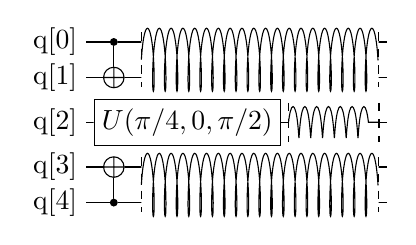
\begin{tikzpicture}
  \begin{yquant}
    qubit q[5];
    cnot q[1] | q[0];
    box {$U(\pi/4, 0, \pi/2)$} q[2];
    cnot q[3] | q[4];
    [name=boxa, draw=none] box {\hspace{80pt}} (q[0], q[1]);
    [name=boxb, draw=none] box {\hspace{27pt}} q[2];
    [name=boxc, draw=none] box {\hspace{80pt}} (q[3], q[4]);
  \end{yquant}
  \spring{boxa}{4mm};
  \spring{boxb}{2mm};
  \spring{boxc}{4mm};
\end{tikzpicture}
\end{document}